%Author: HU Pili
%Start Date: Dec 8, 2012
%Template: ACM Sig template. (preamble comments are moved to the end)

\documentclass{sig-alternate}

\usepackage[tight,footnotesize]{subfigure}
\usepackage{url}
%HU, Pili
%Create: 20120330
%Modify: 20120330
%The unified entry to include in my tutorial series

%HU, Pili
%Create: 20110910
%Modify: 20120330
%purpose of this file is to gather commonly used
%mathematical abbreviations, to speed up writing
%notes

%\usepackage[utf8x]{inputenc}
%\usepackage{ucs}
%\usepackage{amsmath}
%\usepackage{amsfonts}
%\usepackage{amssymb}
%\usepackage{amsthm}
\usepackage{url}
\usepackage{graphicx}

%\usepackage{fancyhdr}
%\pagestyle{fancy}
%\fancyhead{}

%=====Calculus======
%the following commands are not originated by me
%I pick them from http://www-solar.mcs.st-and.ac.uk/~clare/Latex/
%the following line controls the style of patial derivative
%1), use \dfrac, height is larger, looks good. 
%2), use \frac, also work, but space looks limited. 
\newcommand{\myfrac}[2]{\dfrac{#1}{#2}}
\newcommand{\diff}[2]{\myfrac{{\rm d}#1}{{\rm d}#2}}
\newcommand{\ndiff}[3]{\myfrac{{\rm d}^{#3}#1}{{\rm d}#2^{#3}}}
\newcommand{\pdiff}[2]{\myfrac{\partial #1}{\partial #2}}
\newcommand{\npdiff}[3]{\myfrac{\partial^{#3} #1}{\partial #2^{#3}}}
\newcommand{\e}[1]{\ensuremath{{\rm e}^{#1}}}
\newcommand{\ldiff}[2]{\ensuremath{{\rm d}#1/{\rm d}#2}}
\newcommand{\lpdiff}[2]{\ensuremath{\partial#1/\partial#2}}
\newcommand{\lnpdiff}[3]{\ensuremath{\partial^{#3}#1/\partial#2^{#3}}}
\newcommand{\dif}[1]{\mathrm{d}#1}

%20120330
%The reason I don't copy the original file as a whole
%is that it contains too many individually preferred 
%definitions. 
%
%I start with those basic symbols and adapt them in use. 

%=====Matrix======
\newcommand{\tr}[1]{\mathrm{Tr}\left[#1\right]}
\newcommand{\tran}[1]{#1^\mathrm{T}}
\newcommand{\her}[1]{#1^\mathrm{*}}
%The following shorthand of matrix may be convenient. 
%However, it is so short that I'm worried it may 
%collide with something else. I don't use at present.
%\newcommand{\m}[1]{\mathbf{#1}}
\newcommand{\adj}[0]{\mathrm{adj}}
\newcommand{\inv}[1]{#1^{-1}}


%=====Theorem definitions=====
%\newcounter{mytheoremorder}
%\newtheorem{mydef}{Definition}
%\newtheorem{myaxm}{Axiom}
%\newtheorem{mylm}{Lemma}
%\newtheorem{mythm}[mytheoremorder]{Theorem}
%\newtheorem{myprop}[mytheoremorder]{Proposition}
%\newtheorem{myex}{Example}

%=====Optimization====
\DeclareMathOperator*{\argmax}{arg\,max}
\DeclareMathOperator*{\argmin}{arg\,min}
\DeclareMathOperator*{\minimize}{minimize}
\DeclareMathOperator*{\maximize}{maximize}
%\newcommand{\maximize}[0]{\mathrm{Maximize~}}
%\newcommand{\minimize}[0]{\mathrm{Minimize~}}

%=====Probability====
\newcommand{\E}[0]{\mathbb{E}}
\newcommand{\var}[0]{\mathrm{Var}}
\newcommand{\cov}[0]{\mathrm{Cov}}

%=====Quick and Unified Reference====
%20120505
%Usage: \eq{\ref{xxx}}
%The reason I keep "\ref" away from definition, 
%and let user type it every time is that: 
%currently I'm working on Texmaker, and it can 
%trigger a selection panel when the sequence 
%"\ref" is found. Maybe further configuration of 
%texmake can make it do the same thing when the 
%following self-defined sequence is detected.
%This is left for future work. 
\newcommand{\req}[1]{\textbf{Eq~{#1}}}
\newcommand{\rfig}[1]{\textbf{Fig~{#1}}}
\newcommand{\rtbl}[1]{\textbf{Tbl~{#1}}}
\newcommand{\rpg}[1]{\textbf{P~{#1}}}
\newcommand{\rsec}[1]{\textbf{Section~{#1}}}
\newcommand{\ralg}[1]{\textbf{Alg~{#1}}}



\usepackage{glossaries}
\newacronym{sns}{SNS}{Social Networking Services}
\newacronym{osn}{OSN}{Online Social Networks}
\newacronym{dsn}{DSN}{Decentralized Social Network}
\newacronym{msn}{MSN}{Mobile Social Network}
\newacronym{dtn}{DTN}{Delay Tolerant Network}
\newacronym{nfc}{NFC}{Near-Field Communication}
\newacronym{d2d}{D2D}{Device-to-Device}
\newacronym{ppr}{PPR}{Personalized PageRank}
\newacronym{pr}{PR}{PageRank}
\newacronym{xmpp}{XMPP}{Extensible Messaging and Presence Protocol}
\newacronym{roc}{ROC}{Receiver Operating Characteristics}
%\newacronym{roca}{ROCA}{Receiver Operating Characteristics Area}
%\newacronym{auc}{AUC}{Area Under the (ROC) Curve}
\newacronym{auc}{AUC}{Area Under the ROC Curve}
\newacronym{tpr}{TPR}{True Positive Rate}
\newacronym{fpr}{FPR}{False Positive Rate}
\newacronym{ev}{EV}{Escape Vector}
\newacronym{rw}{RW}{Random Walker}
\newacronym{srfe}{SRFE}{SNSRouter Front End}

\begin{document}
\conferenceinfo{
	Please ignore the above and following Copyright statements. 
	It's from the template. 
}{...}
%
% --- Author Metadata here ---
%\conferenceinfo{Have Not Submitted to Conference Yet
%	\footnote{sdfsdfsdfds}
%}{Earth}
%\CopyrightYear{2007} % Allows default copyright year (20XX) to be over-ridden - IF NEED BE.
%\crdata{0-12345-67-8/90/01}  % Allows default copyright data (0-89791-88-6/97/05) to be over-ridden - IF NEED BE.
% --- End of Author Metadata ---

\title{ {\ttlit SNSRouter} -- 
	A Framework for  \\
	Intelligent Message Routing on Heterogeneous SNS
	\titlenote{
		Source codes of the paper and project can be found 
		in the following Github repository. 
		This repository is continuously evolving. 
		\url{https://github.com/hupili/sns-router}
	}
}
%\subtitle{
%	Middleware for SNS's and Flexible Personsalized Ranking Framework
%}
%\subtitle{[Extended Abstract]
%}}

%
% You need the command \numberofauthors to handle the 'placement
% and alignment' of the authors beneath the title.
%
% For aesthetic reasons, we recommend 'three authors at a time'
% i.e. three 'name/affiliation blocks' be placed beneath the title.
%
% NOTE: You are NOT restricted in how many 'rows' of
% "name/affiliations" may appear. We just ask that you restrict
% the number of 'columns' to three.
%
% Because of the available 'opening page real-estate'
% we ask you to refrain from putting more than six authors
% (two rows with three columns) beneath the article title.
% More than six makes the first-page appear very cluttered indeed.
%
% Use the \alignauthor commands to handle the names
% and affiliations for an 'aesthetic maximum' of six authors.
% Add names, affiliations, addresses for
% the seventh etc. author(s) as the argument for the
% \additionalauthors command.
% These 'additional authors' will be output/set for you
% without further effort on your part as the last section in
% the body of your article BEFORE References or any Appendices.

\numberofauthors{1} %  in this sample file, there are a *total*
% of EIGHT authors. SIX appear on the 'first-page' (for formatting
% reasons) and the remaining two appear in the \additionalauthors section.
%
\author{
% You can go ahead and credit any number of authors here,
% e.g. one 'row of three' or two rows (consisting of one row of three
% and a second row of one, two or three).
%
% The command \alignauthor (no curly braces needed) should
% precede each author name, affiliation/snail-mail address and
% e-mail address. Additionally, tag each line of
% affiliation/address with \affaddr, and tag the
% e-mail address with \email.
%
% 1st. author
\alignauthor
    Pili Hu
    \titlenote{\url{http://personal.ie.cuhk.edu.hk/~hpl011/}} \\
    \affaddr{Information Engineering}\\
    \affaddr{The Chinese University of Hongkong}\\
    \affaddr{Shatin, NT, Hongkong}\\
    \email{hupili@ie.cuhk.edu.hk}
}

\maketitle
\begin{abstract}
	Online Social Networks (OSN) has become an essential part of human life today. 
	They also share a very large portion of Internet traffic in terms of Page Visits. 
	Successful OSN's are like Facebook, Twitter, Renren, SinaWeibo, etc. 
	Two of the basic functions are: 1) maintain connections with people; 
	2) read/write updated information in a networked fashion. 

	In this paper, we focus on the function of \textbf{information acquisition and spreading}.
	We build a middleware for heterogeneous Social Network Services (SNS), 
	thus enabling very easy cross-platform message manipulation. 
	Besides those traditional OSN's, we can also abstract RSS, Email, SQLite 
	and more other platforms in the same way. 
	With this middleware, SNSAPI \cite{github_snsapi}, 
	many novel applications can be built and they are ready 
	to be extended to other platforms. 

	We observe that message forwarding is a popular operation on SNS
	and there are many manual cross-platform forwarding behaviours. 
	SNSRouter \cite{github_snsrouter} project aims at developing 
	an easier way to perform cross-platform message forwarding (routing). 
	We propose to leverage combined human and machine intelligence. 
	More specificly, we propose a Rank Preserving Regression (RPR) formulation 
	to personalize incoming messages' ordering. 
	Users with certain programming knowledge can easily add other personalization features. 
	An appropriate ordering saves user's time in reviewing those messages. 
	He/she can then make final forwarding decisions. 

	Evaluation on real traces collected by SNSRouter shows that 
	RPR outputs very good weighting even with preliminary feature extractions. 
	The author of the report, who is not an expert in NLP, can construct those 
	features in one day. 
	This shows the flexibility of our system and algorithm framework. 
\end{abstract}

\category{H.3}{INFORMATION STORAGE AND RETRIEVAL}{Systems and Software}
\category{M.5}{KNOWLEDGE PERSONALIZATION AND CUSTOMIZATION}{Framework}

\terms{System, Algorithm}

\keywords{
	Social Network Services, 
	Middleware, 
	Personalization,
	Rank Preserving Regression
}

\section{Introduction}
\label{sec:Introduction}

Social Network Services minic the real life social networks using modern technology. 
They come in many different forms. 
In this section, we first introduce different Social Network Services
and provide a unified view of them. 
Then we introduce cross-platform message forwarding (routing), 
which motivates the SNSRouter project. 

\subsection{Heterogeneous Social Network Services}
\label{sec:Heterogeneous Social Network Services}

There are many \gls{sns} nowadays.
\rfig{\ref{fig:sns-het}} 
illustrates some of them. 
If we focus on information acquization and spreading
in a networked fashion, 
they can all be casted in thte same way:
\begin{itemize}
	\item \gls{osn}. Examples are like Facebook, Twitter, 
		Renren, SinaWeibo, TecentWeibo in the figure. 
		People form links (either directed or undirected) first
		and information can flow on those links. 
	\item Communication Networks.  
		Examples are like telephone network, SMS network and Email network. 
		On those network, links do not need to be established beforehand. 
		Sender can specify receiver(s) explicitly on the fly. 
	\item Information Sources. 
		Examples are like RSS feeds of blogs and keywords on search engines. 
		When one subscribe to RSS feeds or write a script to monitor the 
		response of a certain keyword search engine, 
		a unidirectional link is established from the information sources to him/her. 
\end{itemize}

As one can see, the only differences are:
1) whether links are formed beforehand;
2) whether links are directed or undirected;
3) whether read/write are allowed or only read (or write) is allowed;
4) whether user authentication/authorization are required.
Currently, there is no efficient way to abstract all these platforms, 
so we see people visting several \gls{sns}'s everyday. 

\begin{figure}[t!]
	\centering
	\includegraphics[width=0.7\linewidth]{../pic/sns-het.pdf}
	\caption{Illustration of Heterogeneous SNS}
	\label{fig:sns-het}
\end{figure}

\subsection{Cross Platform Message Forwarding}
\label{sec:Cross Platform Message Forwarding}

%Instead of being trapped in some platforms, people had better focus on information itself.
%Information shows its value in the process of spreading.
Information spreading in a single domain is natural. 
Many platforms have built-in ``forward'' functions, 
e.g. ``retweet'' on twitter, ``forward'' in email, etc. 
Many researches have also been done for information spreading on a single platform. 
However, cross-platform behavior is a seldom discussed topic. 
We believe this is largely due to lack of mature engineering models
and large collection of data sets. 
Nevertheless, we observe many manual cross-platform behaviours.
For example:

\begin{itemize}
	\item 
	You subscribe to a blog RSS and read a gossip on it.
	The gossip is interesting so you copy and paste it to Renren. 
	%Renren is an OSN, which is typical SNS in our traditional understanding.
	%Blog, from the subscriber's point of view, is also a kind of SNS, but is read-only.
	\item 
	You receive Google Scholar updates on a certain topic by email.
	Once there are some eye-catching new papers, you forward to your colleagues by email.
	%Email is also SNS, where the link is formed dynamically and message is targeted instead of being posted on a wall.
	\item
	Now iPhone 5 is a big event and you want to get latest news about it.
	Instead of following ``inbridge'' at ``twitter'', you can follow ``iphone+5'' at ``baidu''
	(by automatically poll the link: \url{http://www.baidu.com/s?ie=utf-8&wd=iphone+5}). 
	%Traditionally, you follow some guy on Sina Weibo or Twitter.
	%This guy always keeps an eye on big tech news so you are informed of the latest news.
	%Here's an alternative: \url{http://www.baidu.com/s?ie=utf-8&wd=iphone+5}.
	%You can think of ``baidu'' as an SNS, where there are many people who usually give you the updated messages on a certain topic.
	%Of course, after getting the news, you are very likely to forward it to Sina Weibo.
	%(Congratulations! You stand at the frontier now!!)
\end{itemize}

Note the roles people play in the above examples. 
We know Internet routers connect different IP subnet. 
Analogously, those people are routers across different \gls{sns}s. 
The routing job is done manually at preset. 
How about making it automated or semi-automated? 
Can we learn one's preference and use machine intelligence to assit the routing?  

\subsection{Organization}
\label{sec:Organization}

SNSRouter \cite{github_snsapi} is built on a prior work -- SNSAPI \cite{github_snsapi}.
In order to make this document self-contained, 
we will also include SNSAPI in the system design section. 
%SNSAPI and SNSRouter as a whole. 

In 
\rsec{\ref{sec:Related Work}}
, we briefly survey related work. 
In 
\rsec{\ref{sec:Philosophy}}
, we disucss design philosophy of SNSAPI and SNS-Router. 
In 
\rsec{\ref{sec:System Framework}}
, we present the system framework. 
In 
\rsec{\ref{sec:Formulation}}
, we formulate the personalization problem as Ranking Preserving Regression. 
In
\rsec{\ref{sec:Algorithm Design}}
, we transform the problem and propose to use 
Stochastic Gradient Descent (SGD) as the training algorithm. 
In 
\rsec{\ref{sec:Evaluation}}
we evaluate all aspects of our algorithm framework:
efficiency, accuracy, robustness, and flexibility. 
Last, we conclude this paper in 
\rsec{\ref{sec:Conclusion}}
and share our visions on future works in 
\rsec{\ref{sec:Future Work}}
.

%    sec:Related Work
%    sec:Philosophy
%    sec:System Framework
%    sec:Formulation
%    sec:Impossibility of Complete Auto Forwarding
%    sec:The Problem of Classification
%    sec:Regression Formulation
%    sec:Algorithm Design
%    sec:Induce Preference Relations on Graph
%    sec:Straight Optimization Solver
%    sec:Problem Transformation
%    sec:Gradient Descent
%    sec:Stochastic Gradient Descent
%    sec:Evaluation
%    sec:HU's Data Set
%    sec:Criterion
%    sec:Efficiency and Complexity
%    sec:Robustness
%    sec:Case Study -- Add ``echo'' Feature
%    sec:Conclusion
%    sec:Future Work

% ==== past paragraphs in proposal ====
%We observe many such cross-domain forwarding behaviors everyday! 
%However, we lack abstraction of those platforms and differently formatted messages. 
%Users don't have a unified way to perform easy forwarding. 
%Researchers don't have cross-domain data for study. 
%We take an initial step towards this direction. 
%The open-source SNSAPI project develops a middle ware to unify different SNS (OSN, RSS, email, etc).
%Different SNSs are abstracted in the form of channel and they support primitives like auth(), read(), write().
%The SNSAPI project is at its infancy.
%We'll spend some time contributing to SNSAPI but do not count it in the SNSRouter project.
%The SNSRouter project lies on SNSAPI (App layer in SNSAPI terminology). 
%We'll focus on prototyping an easy way to route cross-domain messages. 
%On this prototype system, we'll be able to collect trace data. 
%Using this cross-domain routing data, we can train algorithms to intelligently make forwarding decisions.
%We plan to leverage topology (e.g. come from whom), 
%content (e.g. the topic) and context (e.g. time of day / location of user) features.
%It's worth to note that SNSAPI framework enables very flexible usage.
%One can configure an archive channel (e.g. email) 
%and write all messages he like there for future retrieval. 
%In this case, the routing (originally can be multiple-input-multiple output) 
%degrades to a multiple-in-single-out personal recommender system.
%To make things tractable, we'll start with the recommender algorithm using all three kinds of features.

\section{Related Work}
\label{sec:Related Work}

From the system aspect, some Internet resource aggregation services are related. 
From the algorithm aspect, some personalization services are related. 
In this section, we briefly survey those services. 

\subsection{Aggregation Services}
\label{sec:Aggregation Services}

There are many aggregation services on the Internet. 
Some of them focus on dealing with a certain type of sources, 
e.g. Google Reader for RSS feeds. 
Some of them can aggregate heterogeneous sources, 
like ifttt \cite{ifttt} and Yahoo Pipes \cite{yahoo_pipes}. 

ifttt abstracts services on the Internet by ``channel'' 
(we borrow this term in SNSAPI), 
e.g. Facebook, Twitter, RSS, SMS, etc. 
Users can define forwarding rules (called ``recipe'' on ifttt)
in this manner:
IF This happens, Then do That (IFTTT). 
This service is very handy for normal users who simply want to bridge several services, 
e.g. publish status on Facebook and the message is automatically forwarded to Twitter. 
ifttt supports a wide spectrum of platforms, 
but there is little flexibility for user to build advanced rules. 

Yahoo Pipes (YP), on the contrary, supports less platforms but allows somewhat advanced rules. 
YP focus on the traditional web, so operations like 
fetching webpage, RSS feeds and CVS table are supported. 
In the pipe construction UI, users can drag sources 
and logic modules (e.g. condition, loop, etc) to the design board
and connect them using ``pipe''.
In the Web1.0 world, YP could be a good aggregator. 
However in the web2.0 world, 
User Generated Content (UGC) is dominating 
and it is full of noise. 
Simple constructions provided by YP is far from enough. 
e.g. forward a certain topic RSS entries to somewhere else. 

\subsection{Personalization with Machine Intelligence}
\label{sec:Personalization with Machine Intelligence}

One major problem of those \gls{sns}'s is that there are too 
many messages flowing throughout the network. 
Even the data rate within one's personal view is too large for human to process efficiently. 
%The noise level is too high to prevent people from 
%acquiring information efficiently. 
%is significantly lowered. 
%efficiency of 
Besides filtering out noise, one also want to prioritize the display of messages 
so that messages can be processed by human in descending order of their importance. 
Different users have different preference so personalization is needed. 
Towards this end, many service providers also develop their own 
machine learning algorithms to help users personalize the incoming messages. 

Personalized incoming message ranking is of its own research interest 
even in the case of single platform. 
For example, SinaWeibo by default presents incoming messages 
in reverse chronological order. 
Users can enable ranked view and obtain a probably more informative timeline. 
For another example, GMail classifies incoming messages 
into ``important'' and ``ordinary'' types 
so that users can process ``important'' messages first. 

Existing approches focus more on developing better algorithms. 
Training data is obtained mostly by implicit feedback, 
e.g. how long a user stay on one message. 
User engagement in the training cycle is very low. 
Thus the degree of personalization is also low. 
Besides, those service providers target mass audience
and provide no flexibility for people who understands how to program. 
For example, one may suffer spontaneously from someone's overwhelming messages. 
The common practice is to block his/her mesages (not unlink the user). 
However, service providers ususally set an upperbound on the number users blocked, 
e.g. 5 for Renren and 15 for SinaWeibo. 
One needs to upgrade his/her account to paid member in order to grow the upperbound. 
Anyone who know programming agrees that blocking specified users
is a very simple task given proper programming interface. 
To avoid blocking spontaneous noise sources permanently, 
one can also set some timeout logic or probabilistic blocking logic. 
However, all of those simple operations are not possible in current services. 

On one hand, existing personalization approaches try to 
solve harder than necessary problems with little user side knowledge. 
On the other hand, some simple personalization demand 
can not be implemented by the users. 

\section{Philosophy}
\label{sec:Philosophy}

In this section, we discuss the design philosophy 
of our system framework and algorithm framework. 
In a word, we pursue simple but effective approaches
which leverage human and machine intelligence simultaneously. 

\begin{itemize}
	\item \textbf{Focus on solving 80\% problems}. 
		The Pareto Principle \cite{wiki_pareto} tells us that 
		(qualitively) one only needs 20\% effort to solve 80\% problems; 
		In order to solve the rest 20\% problems, he/she needs to 
		spend the other 80\% time. 
		Example: conecptually, we only abstract three methods for \gls{osn}, 
		namely \textbf{read}, \textbf{write} and \textbf{auth}. 
		The three methods can cover more than 80\% functions one need on an \gls{osn}. 
		They are also universal across many other \gls{sns}. 
		However, in order to abstract many platform specific functions, 
		we need much more time, but those functions may be seldom used 
		in our cross-platform settings. 
	\item \textbf{Keep It Simple and Stupid (KISS)} \cite{wiki_kiss}. 
		Whenever possible, we prefer simpler solutions. 
		Common and hard cut rules will be implemented directly with configurable interface. 
		e.g. one can configure some channels to be read-only and others to be write-only directly. 
		We do not need to ``learn'' such preference through user interaction. 
		%2) When simpler features are effective enough, we do not consider advanced features. 
		%3) When simpler 
		This principle also applies to our algorithm framework design, 
		i.e. When simpler features are effective enough, we do not consider advanced features;
		When linear combination is good enough, we do not bother to look at non-linear combinations. 
	\item \textbf{Combine human and machine intelligence}. 
		In \rsec{\ref{sec:Related Work}} we discussed the current approaches adopted by 
		both industry and research communities. 
		Machine learning algorithms are asked to do much harder tasks than necessary. 
		For one extreme example, one can put all bits of a message 
		(sender, text, time, etc) into one very long vector as feature. 
		If we have a very powerful machine learning algorithm, it may be able to 
		learn what factor is important to personalize one's messages and rank them reasonably. 
		Such algorithm, even exists, will be very costly. 
		However, the user speaks louder than any statistical clues.  
		If one user always prefer longer messages than shorter message, 
		he/she just put the length of message into the feature vector and that is enough. 
		We will discuss more in the formulation section. 
		%A simple algorithm can learn such preference. 
	\item \textbf{Stay open with existing services}. 
		We never want to solve a full stack of problem. 
		Many problems are already solved (probably in a degraded way). 
		We encourage users to take advantage of existing services
		rather than reinventing wheels. 
		Example: I want to forward important messages from \gls{osn} to 
		my cellphone through SMS. 
		I will not try hard to enable ``SMS platform'' on SNSAPI. 
		Instead, I will build the intelligence which filers out ``important'' messages using SNSAPI
		and then output those messages to an RSS file. 
		Later on ifttt, I just add a straight forwarding recipe from the RSS file 
		to my cellphone through SMS. 
	\item \textbf{Trade execution efficiency for developing efficiency}. 
		Many of the codes in this project are not optimized. 
		There is no incentive to optimize them unless the execution 
		time is out of human tolerable range. 
		We prefer to make the codes extensible rather than running fast. 
\end{itemize}

\section{System Framework}
\label{sec:System Framework}

The system is divited into two parts:
\begin{itemize}
	\item SNSAPI is the middleware to interface with 
		heterogeneous \gls{sns}'s. 
		Other developers can write ``plugin'' to enable new platform. 
		Applications built on SNSAPI is readily available for future new platforms. 
	\item \gls{srfe} is the web-based UI for SNSRouter. 
		Users can accomplish authorization, view incoming messages, post messages, 
		and forward messages using \gls{srfe}. 
		If ranking algorithm is enabled in the configuration, 
		ranked timeline is also presented in \gls{srfe}. 
		\gls{srfe} can be run wherever Python is supported. 
\end{itemize}

\subsection{SNSAPI Architecture}
\label{sec:SNSAPI Architecture}

\begin{figure}[t!]
	\centering
	\includegraphics[width=0.7\linewidth]{../pic/snsapi-arch.pdf}
	\caption{SNSAPI Architecture}
	\label{fig:snsapi-arch}
\end{figure}

\rfig{\ref{fig:snsapi-arch}} illustrates the system framework of SNSAPI. 
There are conceptually three layers:
\begin{itemize}
	\item Interface Layer. 
		SNSBase is the base class for all kinds of \gls{sns}. 
		One can derive the base class to implement real logic that interfaces with those platforms. 
		In SNSAPI terminology, the modules containing derived classes are called ``plugin'';
		the derived classes are called ``platform''; 
		the instance of the classes are called ``channel''. 
		Message and message list types are also defined in this layer. 
		We make all the interfacing types json-serializable and pickle-able, 
		so the communications inside and outside SNSAPI are very easy. 
	\item Physical Layer. 
		There are many common operations when one interfaces with different \gls{sns}'s. 
		We implement them in the Physical layer so that plugin authors do not need to 
		build all the logics from scratch. 
		Examples are like, HTTP request/response, OAuth, Error definition, etc. 
		Many third party modules are used in this layer. 
		To keep flexibilty, we provide wrapper class for most third party modules, 
		so that one can subsitute (part of) them with better ones easily. 
	\item Application Layer. 
		Application authors can directly use classes in the interface layer. 
		e.g. write an auto-reply script by using RenrenStatus (derived from SNSBase);
		only a dozon of lines are needed. 
		However, when one want to operate a large collection of channels, this is not efficient. 
		To avoid frequently repeated work, we develop a container class called ``SNSPocket''. 
		Pocket can hold a collection of channels and perform batch operation 
		with some simple configurable rules. 
		For most applications, Pocket should be the Service Access Point (SAP) to SNSAPI. 
		When there are new channels, users can enable them by configuration
		and no active involvement from the App developer is needed. 
\end{itemize}

In the Application Layer, we also include one Command Line Interface (CLI) -- ``SNSCLI''. 
The reason comes in three folds. 
First, SNSCLI is more appropriate for initial trials. 
It is run in a Python interactive shell and usage is also natural to non-Python users. 
Second, for App developer, SNSCLI can be used for debugging purpose. 
Third, if non-Python developers want to use SNSAPI, SNSCLI can serve as the SAP. 
Commands are piped in SNSCLI using STDIN and results are obtained from STDOUT. 
\rfig{\ref{fig:snscli}} is the screenshot of a running SNSCLI. 

\begin{figure}[t!]
	\centering
	\includegraphics[width=0.7\linewidth]{../pic/snsapi-screen-1.pdf}
	\caption{Command Line Interface of SNSAPI}
	\label{fig:snscli}
\end{figure}

We remark that the above is just conceptual illustration of the SNSAPI framework. 
File level details are avoided in this document as they are distraction from our main topic. 
Interested readers can go to our project repository \cite{github_snsapi} 
and consult the developer's wiki. 

\subsection{SNSRouter Architecture}
\label{sec:SNSRouter Architecture}

In SNSAPI terminology, SNSRouter is an Application bulit upon it. 
As we are Python developers, we choose to use Pocket class as the SAP to SNSAPI. 
The system part, i.e. \gls{srfe}, can be divided into three parts:
\begin{itemize}
	\item Web UI. 
		At the start time of \gls{srfe}, we face different choices of UI:
		desktop software or web services. 
		We choose web UI because we want \gls{srfe} able to be accessed from any platforms. 
		Another consideration is that the web UI is easy to be extended 
		so that it provides RESTful API to downflow applications. 
		To build \gls{srfe}, we need HTTP request handler, 
		URL routing, and simple template engine. 
		There are many micro frameworks available in Python like cherrypy, flask, and bottle. 
		We choose bottle mainly because of its single file property. 
		This makes it easy to distribute along with SNSRouter so that minimum dependencies are required. 
	\item Message Queue. 
		If Web UI interface with SNSAPI directly, the response cycle will be very long. 
		This is because SNSAPI's application programming model is synchronous, 
		e.g. pocket invokes certain method of all channels and wait for response one by one. 
		We believe this it's the App developers job to choose 
		multi-threading or multi-processing solutions. 
		In \gls{srfe}, we implement an asynchronous message queue, which is running in the backend. 
		It polls each channel periodically and store messages in a local SQLite database. 
		Request from Web UI is routed to the Message Queue so that response cycle is shortened. 
	\item Ranking. 
		Ranking can be enabled or disabled by configuration. 
		Ranking module has interface with Queue. 
		When enabled, incoming messages get their scores. 
		From the Web UI, users can reach ranked timeline by asking 
		the Message Queue to sort messages in descending order of score. 
		Feature extraction and auto weighting (learner) logic is implemented in Ranking module. 
\end{itemize}

\rfig{\ref{fig:srfe_hometimeline}} shows a screen shot of 
ordinary timeline (reverse chronological order). 
Users can mark a message as "seen" so that it won't appear later in the timeline. 
"seen" flag will be an important part in the training data later. 
Below each message is a set of user defined tags. 
Different user can have different criterion and interpretation of those tags. 
Below tags is the forwarding panel. 
Users can add his/her own comments and forward the new message to all other platforms. 
This is further configurable (e.g. which tag to forward to which platform). 
\rfig{\ref{fig:srfe_rankedtimeline}} shows the screen shot 
of ranked timeline at the same time. 
The author's opinion on those messages are depicted in thsoe screenshots. 
From this pair of screenshots, we can see that ranked version is much cleaner
so that user can make forwarding decisions more efficiently 
(Quantitative measures are presented in the evaluation section). 

\begin{figure*}[t!]
	\centering
	\subfigure[Original Home Timeline on SRFE]{%
	\label{fig:srfe_hometimeline}
	\includegraphics[width=0.4\linewidth]{../pic/srfe-screen-1.pdf}
	}%   
	\subfigure[Ranked Home Timeline on SRFE]{%
	\label{fig:srfe_rankedtimeline}
	\includegraphics[width=0.4\linewidth]{../pic/srfe-screen-2.pdf}
	}%   
	\caption{Original v.s. Ranked Timeline. Screen shot taken at around Dec 3, 11:30am}
\end{figure*}

%\begin{figure}[t!]
%	\centering
%	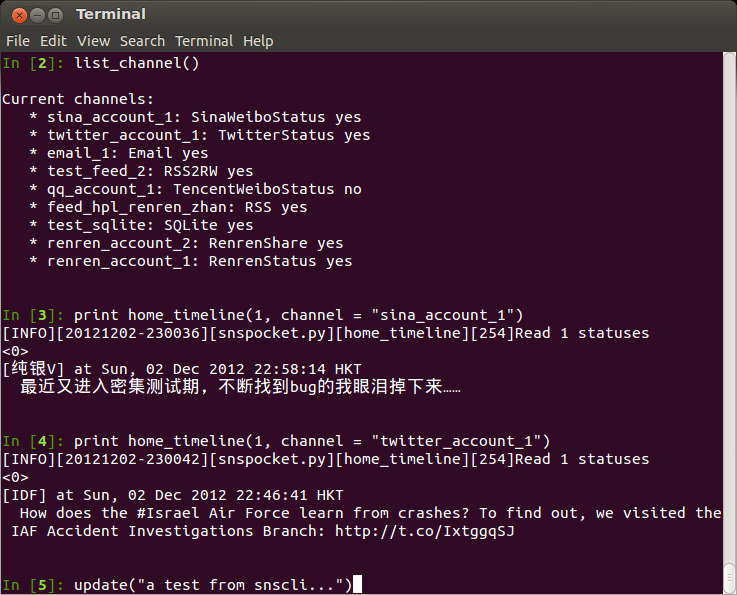
\includegraphics[width=0.7\linewidth]{../pic/snscli.png}
%	\caption{Command Line Interface of SNSAPI}
%\end{figure}
%
%%\begin{figure}[t!]
%%	\centering
%%	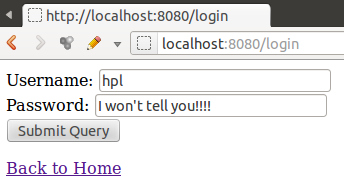
\includegraphics[width=0.7\linewidth]{../pic/srfe_login.png}
%%	\caption{Command Line Interface of SNSAPI}
%%\end{figure}
%
%\begin{figure}[t!]
%	\centering
%	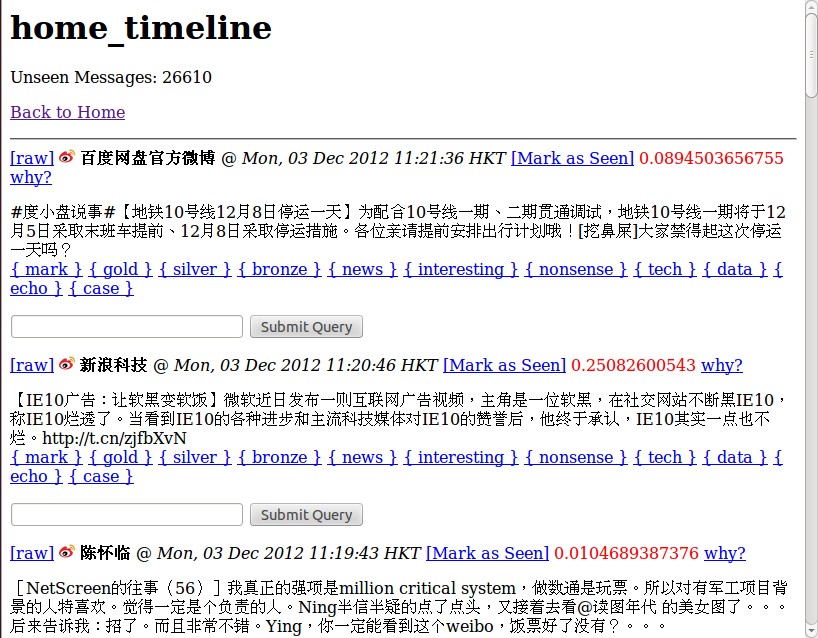
\includegraphics[width=0.7\linewidth]{../pic/srfe_home_timeline.png}
%	\caption{Command Line Interface of SNSAPI}
%\end{figure}
%
%\begin{figure}[t!]
%	\centering
%	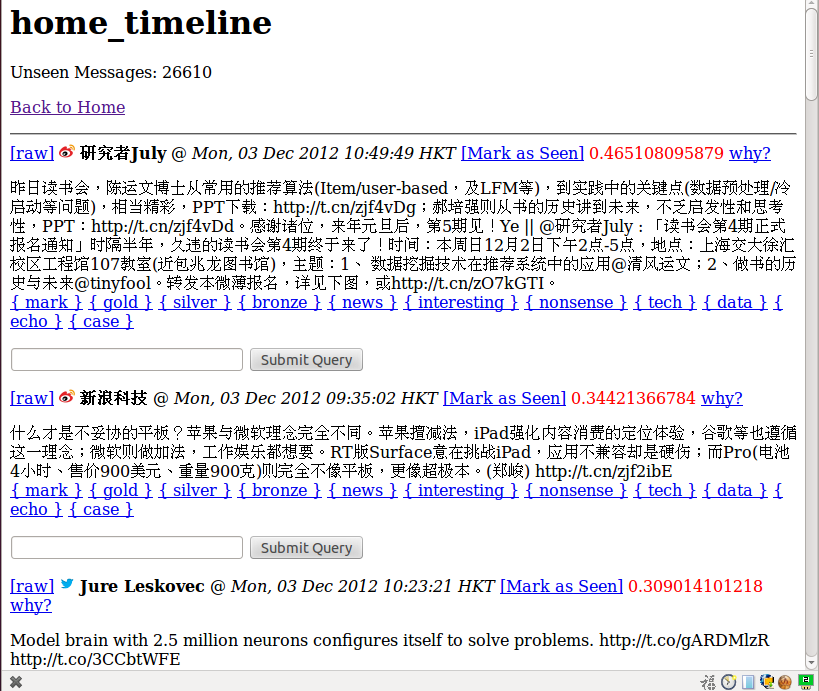
\includegraphics[width=0.7\linewidth]{../pic/srfe_ranked_timeline.png}
%	\caption{Command Line Interface of SNSAPI}
%\end{figure}


\section{Formulation}
\label{sec:Formulation}

In this section, we discuss how we formulate a personalized ranking problem. 
Bear in mind that our ultimate goal is to make 
cross-platform message routing efficient. 
Now the engineering problem has been solved by SNSAPI and \gls{srfe}. 
Next is to design proper machine learning algorithms to make this done automatically. 
In this section, we first discuss the impossibility of 
complete auto forwarding algorithms. 
Then we discuss the problems arise from classification formulation. 
Last, we propose a regression model with user preference constraints. 

\subsection{Impossibility of Complete Auto Forwarding}
\label{sec:Impossibility of Complete Auto Forwarding}

\subsection{The Problem of Classification Formulation}
\label{sec:The Problem of Classification}

\begin{equation}
	\tran{X} = [x_1, x_2, \ldots, x_N]
\end{equation}

Analyze the result of Logit Classifier and J48. 

\begin{itemize}
	\item 
	Hard cut. Do not output a likelihood.
	\item 
	Human can only process sequentially. 
	Accurate classification is not needed.
\end{itemize}

\subsection{Regression Formulation}
\label{sec:Regression Formulation}

\begin{eqnarray}
	\minimize_{y,w} && ||y - Xw||_2^2 \\
	\text{s.t.} && y_i > y_j, \; \forall (i,j) \in E
\end{eqnarray}

\section{Algorithm Design}
\label{sec:Algorithm Design}

\subsection{Induce Preference Relations on Graph}
\label{sec:Induce Preference Relations on Graph}

\begin{figure}[t!]
	\centering
	\includegraphics[width=0.7\linewidth]{../pic/graph-induction.pdf}
	\caption{Graph Induction Illustration}
\end{figure}

\subsection{Straight Optimization Solver}
\label{sec:Straight Optimization Solver}

Existing solvers?
Ordinal regression?
Isotonic regression?

\subsection{Problem Transformation}
\label{sec:Problem Transformation}

Constraint as objective: (indicator function)

\begin{eqnarray}
	\minimize_{y,w} && \sum_{(i,j) \in E} 1 - I[y_i > y_j] \\
	\text{s.t.} && y = Xw
\end{eqnarray}

Approximation by Sigmoid:

\begin{eqnarray}
	\minimize_{y,w} && f(w) \equiv \sum_{(i,j) \in E} 1 - \text{Sigmoid}[y_i > y_j] \\
	\text{s.t.} && y = Xw
\end{eqnarray}


\subsection{Gradient Descent}
\label{sec:Gradient Descent}

\begin{equation}
	\nabla f(w) = \sum_{(i,j) \in E} \nabla f_{ij}(w) 
\end{equation}

Observation: full gradient is the summation of
per pair partial gradient. 

\begin{equation}
	\nabla f_{ij}(w) = \beta (1-S[y_i - y_j])S[y_i-y_j](x_j-x_i)
\end{equation}

\subsection{Stochastic Gradient Descent}
\label{sec:Stochastic Gradient Descent}


\section{Evaluation}
\label{sec:Evaluation}

\subsection{HU's Data Set}
\label{sec:HU's Data Set}

\subsection{Criterion}
\label{sec:Criterion}

Kendall's tau correlation coefficient. 

\begin{equation}
	K = \frac{\sum_{(i,j)}{I[y_i>y_j]} - \sum_{(i,j)}{I[y_j>y_i]}}{|E|}
\end{equation}

\subsection{Efficiency and Complexity}
\label{sec:Efficiency and Complexity}

\begin{table}[t!]
	\caption{Features}
	\centering
	\begin{tabular}{|l|p{0.6\linewidth}|}
		\hline
		Name & Description \\
		\hline
		noise & Random variable [0,1]\\
		echo & Whether the message is from myself\\
		contain\_link & Whether the message contain text link\\
		topic\_interesting & TF*IDF for {interesting}\\
		topic\_tech & TF*IDF for {mark}{gold}{silver}{bronze}\\
		topic\_news & TF*IDF for {news}\\
		topic\_nonsense & TF*IDF for {nonsense}{shit}\\
		user\_interesting & As above; regard ``user'' as ``term''\\
		user\_tech & As above\\
		user\_news & As above\\
		user\_nonsense & As above\\
		text\_len & Length of all message (original + retweet)\\
		text\_len\_clean & Length without face icon, link, @xxx, and puctuation\\
		text\_orig\_len & Length of original message\\
		\hline
	\end{tabular}
\end{table}

\begin{table}
	\centering
	\caption{Training with SGD}
	\begin{tabular}{|c|c|c|c|}
	\hline
	Item & 1. & 2. & 3. \\
	\hline
	\# of rounds of SGD & 200,000 & 400,000 & 1,000,000\\
	Wall clock time & 32.63s & 60.81s & 159.57s\\
	Kendall's score (training) & 0.8178 & 0.8349 & 0.8414\\
	Kendall's score (testing) & 0.7598 & 0.7758 & 0.7865\\
	\hline
	\end{tabular}
\end{table}

Straight SGD implemented in SNSRouter project. Code has not been optimized.

\begin{itemize}
	\item Scale linearly
	\item Online learning is possible
	\item Easy configuration
	\item Easy to add new features
\end{itemize}

\subsection{Robustness}
\label{sec:Robustness}

Start with already trained weights for
other features. Largest magnitude is <10.

Inject 1 noise feature, picking U[0,1]. Init
it’s weights by 10.

\begin{table}
	\begin{tabular}{|c|c|c|c|}
		\hline 
		& Init & Round=200K & Round=400K \\
		\hline 
Kendall & 0.0772 & 0.5435 & 0.8060 \\
 w(noise) & 10.0 & 1.3407 & -0.0132 \\
		\hline
	\end{tabular}
\end{table}

\subsection{Case Study -- Add ``echo'' Feature}
\label{sec:Case Study -- Add ``echo'' Feature}

Most platforms will echo the
message you post there, but they
do not give you more information.
We want to SOFTLY cancel them.

Cancel echo:

1. Add tag ``echo''

2. Specify preference

3. Add feature

4. AUTO train weights

\begin{figure}[h!]
	\centering
	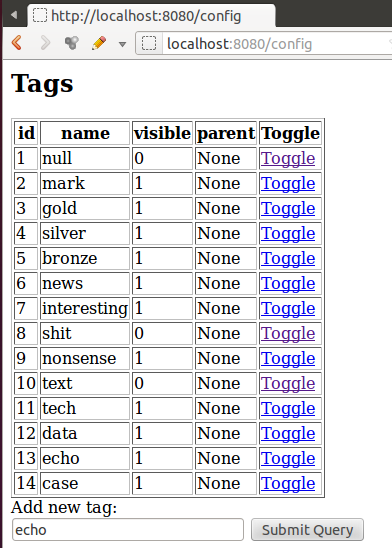
\includegraphics[width=0.7\linewidth]{../pic/echo_add_tag.png}
	\caption{Add New Tag on Config Panel}
\end{figure}

\begin{figure}[h!]
	\centering
	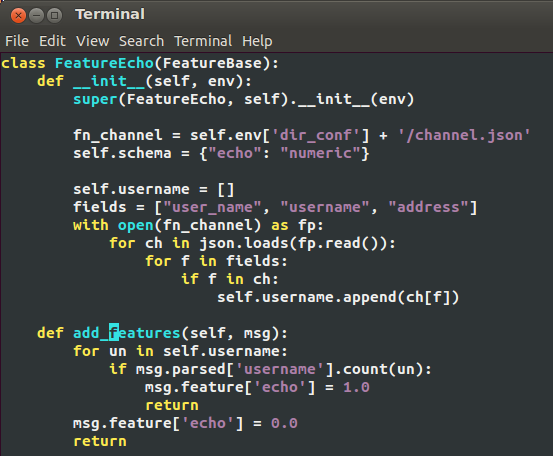
\includegraphics[width=0.7\linewidth]{../pic/echo_feature.png}
	\caption{Add New Tag on Config Panel}
\end{figure}

\begin{figure}[h!]
	\centering
	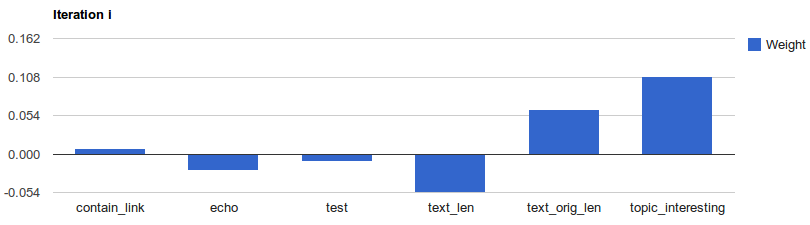
\includegraphics[width=0.7\linewidth]{../pic/echo_gd_i.png}
	\caption{Add New Tag on Config Panel}
\end{figure}

\begin{figure}[h!]
	\centering
	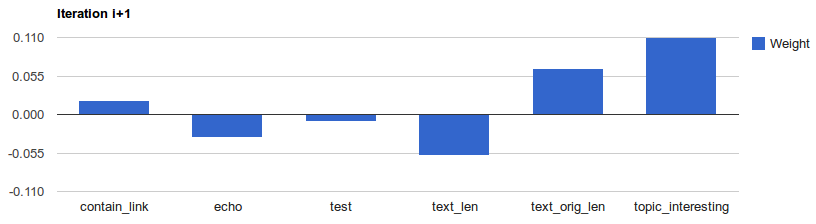
\includegraphics[width=0.7\linewidth]{../pic/echo_gd_i1.png}
	\caption{Add New Tag on Config Panel}
\end{figure}

\begin{figure}[h!]
	\centering
	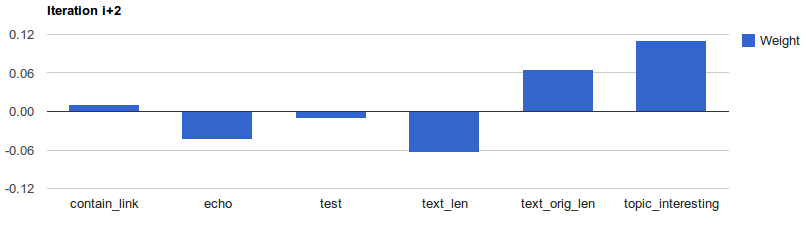
\includegraphics[width=0.7\linewidth]{../pic/echo_gd_i2.png}
	\caption{Add New Tag on Config Panel}
\end{figure}

\begin{figure}[h!]
	\centering
	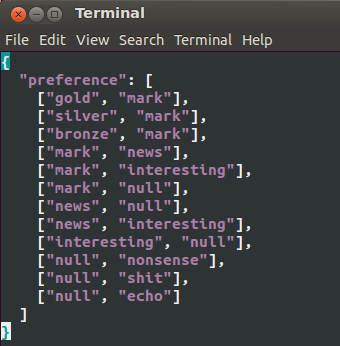
\includegraphics[width=0.7\linewidth]{../pic/echo_preference.png}
	\caption{Add New Tag on Config Panel}
\end{figure}

\begin{figure}[h!]
	\centering
	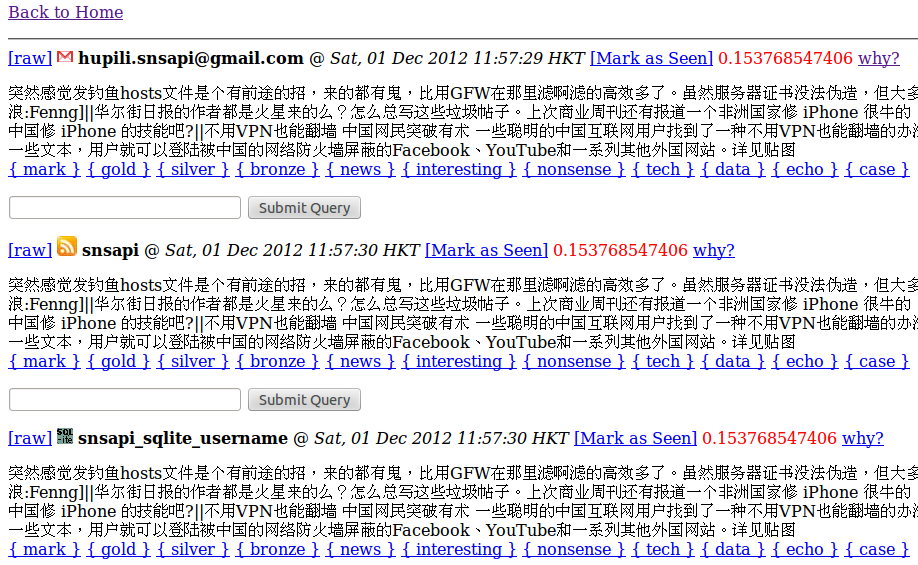
\includegraphics[width=0.7\linewidth]{../pic/echo_ranked_timeline_before.png}
	\caption{Add New Tag on Config Panel}
\end{figure}


The weight of ``echo'' feature goes down iteration by iteration. Messages with ``echo=1''
will be ranked lower. This is auto learned by our RPR-SGD framework.

\section{Conclusion}
\label{sec:Conclusion}

\begin{itemize}
	\item A middleware for different SNS
	\item A portable web frontend
	\item Real data collection (1+ month)
	\item A flexible algorithm framework (RPR-SGD)
	\item Sample feature extraction modules
\end{itemize}



\section{Future Work}
\label{sec:Future Work}

\subsection{System}
\label{sec:fu_System}

\begin{itemize}
	\item RESTful interface for all components.
		e.g. one can outsource computationally
		intensive training to other servers
	\item SNSRouter as a platform (of SNSAPI).
		e.g. can be used to aggregate multiple
		channels. 
	\item ``FeatureStore'' and ``LearnerStore''. 
		Boost community developing and sharing of 
		personalization technique. 
\end{itemize}

\subsection{Algorithm}
\label{sec:fu_Algorithm}

\begin{itemize}
	\item Add regularization to alleviate overfiting. 
	\item Advanced feature extraction.
	\item SGD can do online training.
	e.g. one sample in, derive some pairs, do
	SGD on those pairs.
	Naturally time sliding.
	\item Code optimization of SGD. 
\end{itemize}

\subsection{Evaluation}
\label{sec:fu_Evaluation}

More subjective tests are to be done:

\begin{itemize}
	\item We argue the algorithm framework is easy to personalize. 
		In the future work, we'll invite more developers 
		who are not machine learning experts to test our system. 
\end{itemize}

\section*{Acknowledgements}
\label{sec:Acknowledgements}

We would like to thank Junbo Li from BUPT, 
the cofounder of SNSAPI, 
which is the base of SNSRouter project. 
We also highly appreciate people who answered our 
technical questions on StackOverflow. 

\bibliographystyle{abbrv}
\input{../reference/gen_bib.bbl}

\appendix 

\section{Data}
\label{sec:Data}

\section{Classification}
\label{sec:Classification}

\subsection{Logit Classifier}
\label{sec:Logit Classifier}

\subsection{J48 Decision Tree}
\label{sec:J48 Decision Tree}

A sample branch for mark (3.0/1.0):

\begin{Verbatim}
   topic_news <= 0.00603 
&& topic_tech <= 0.041455
&& topic_interesting <= 0.042225 
&& topic_nonsense <= 0.010593 
&& text_len > 0.12 
&& id <= 30634 
&& user_tech <= 0.010894 
&& text_len_clean <= 0.0575
&& user_tech > 0.001621
\end{Verbatim}

\section{Executive Summary of SNSRouter Usage}
\label{sec:Executive Summary of SNSRouter Usage}




%============== Following are sample lines from the template =================

% This is "sig-alternate.tex" V2.0 May 2012
% This file should be compiled with V2.5 of "sig-alternate.cls" May 2012
%
% This example file demonstrates the use of the 'sig-alternate.cls'
% V2.5 LaTeX2e document class file. It is for those submitting
% articles to ACM Conference Proceedings WHO DO NOT WISH TO
% STRICTLY ADHERE TO THE SIGS (PUBS-BOARD-ENDORSED) STYLE.
% The 'sig-alternate.cls' file will produce a similar-looking,
% albeit, 'tighter' paper resulting in, invariably, fewer pages.
%
% ----------------------------------------------------------------------------------------------------------------
% This .tex file (and associated .cls V2.5) produces:
%       1) The Permission Statement
%       2) The Conference (location) Info information
%       3) The Copyright Line with ACM data
%       4) NO page numbers
%
% as against the acm_proc_article-sp.cls file which
% DOES NOT produce 1) thru' 3) above.
%
% Using 'sig-alternate.cls' you have control, however, from within
% the source .tex file, over both the CopyrightYear
% (defaulted to 200X) and the ACM Copyright Data
% (defaulted to X-XXXXX-XX-X/XX/XX).
% e.g.
% \CopyrightYear{2007} will cause 2007 to appear in the copyright line.
% \crdata{0-12345-67-8/90/12} will cause 0-12345-67-8/90/12 to appear in the copyright line.
%
% ---------------------------------------------------------------------------------------------------------------
% This .tex source is an example which *does* use
% the .bib file (from which the .bbl file % is produced).
% REMEMBER HOWEVER: After having produced the .bbl file,
% and prior to final submission, you *NEED* to 'insert'
% your .bbl file into your source .tex file so as to provide
% ONE 'self-contained' source file.
%
% ================= IF YOU HAVE QUESTIONS =======================
% Questions regarding the SIGS styles, SIGS policies and
% procedures, Conferences etc. should be sent to
% Adrienne Griscti (griscti@acm.org)
%
% Technical questions _only_ to
% Gerald Murray (murray@hq.acm.org)
% ===============================================================
%
% For tracking purposes - this is V2.0 - May 2012


%\section{Introduction}
%The \textit{proceedings} are the records of a conference.
%ACM seeks to give these conference by-products a uniform,
%high-quality appearance.  To do this, ACM has some rigid
%requirements for the format of the proceedings documents: there
%is a specified format (balanced  double columns), a specified
%set of fonts (Arial or Helvetica and Times Roman) in
%certain specified sizes (for instance, 9 point for body copy),
%a specified live area (18 $\times$ 23.5 cm [7" $\times$ 9.25"]) centered on
%the page, specified size of margins (1.9 cm [0.75"]) top, (2.54 cm [1"]) bottom
%and (1.9 cm [.75"]) left and right; specified column width
%(8.45 cm [3.33"]) and gutter size (.83 cm [.33"]).
%
%The good news is, with only a handful of manual
%settings\footnote{Two of these, the {\texttt{\char'134 numberofauthors}}
%and {\texttt{\char'134 alignauthor}} commands, you have
%already used; another, {\texttt{\char'134 balancecolumns}}, will
%be used in your very last run of \LaTeX\ to ensure
%balanced column heights on the last page.}, the \LaTeX\ document
%class file handles all of this for you.
%
%The remainder of this document is concerned with showing, in
%the context of an ``actual'' document, the \LaTeX\ commands
%specifically available for denoting the structure of a
%proceedings paper, rather than with giving rigorous descriptions
%or explanations of such commands.
%
%\section{The {\secit Body} of The Paper}
%Typically, the body of a paper is organized
%into a hierarchical structure, with numbered or unnumbered
%headings for sections, subsections, sub-subsections, and even
%smaller sections.  The command \texttt{{\char'134}section} that
%precedes this paragraph is part of such a
%hierarchy.\footnote{This is the second footnote.  It
%starts a series of three footnotes that add nothing
%informational, but just give an idea of how footnotes work
%and look. It is a wordy one, just so you see
%how a longish one plays out.} \LaTeX\ handles the numbering
%and placement of these headings for you, when you use
%the appropriate heading commands around the titles
%of the headings.  If you want a sub-subsection or
%smaller part to be unnumbered in your output, simply append an
%asterisk to the command name.  Examples of both
%numbered and unnumbered headings will appear throughout the
%balance of this sample document.
%
%Because the entire article is contained in
%the \textbf{document} environment, you can indicate the
%start of a new paragraph with a blank line in your
%input file; that is why this sentence forms a separate paragraph.
%
%\subsection{Type Changes and {\subsecit Special} Characters}
%We have already seen several typeface changes in this sample.  You
%can indicate italicized words or phrases in your text with
%the command \texttt{{\char'134}textit}; emboldening with the
%command \texttt{{\char'134}textbf}
%and typewriter-style (for instance, for computer code) with
%\texttt{{\char'134}texttt}.  But remember, you do not
%have to indicate typestyle changes when such changes are
%part of the \textit{structural} elements of your
%article; for instance, the heading of this subsection will
%be in a sans serif\footnote{A third footnote, here.
%Let's make this a rather short one to
%see how it looks.} typeface, but that is handled by the
%document class file. Take care with the use
%of\footnote{A fourth, and last, footnote.}
%the curly braces in typeface changes; they mark
%the beginning and end of
%the text that is to be in the different typeface.
%
%You can use whatever symbols, accented characters, or
%non-English characters you need anywhere in your document;
%you can find a complete list of what is
%available in the \textit{\LaTeX\
%User's Guide}\cite{Lamport:LaTeX}.
%
%\subsection{Math Equations}
%You may want to display math equations in three distinct styles:
%inline, numbered or non-numbered display.  Each of
%the three are discussed in the next sections.
%
%\subsubsection{Inline (In-text) Equations}
%A formula that appears in the running text is called an
%inline or in-text formula.  It is produced by the
%\textbf{math} environment, which can be
%invoked with the usual \texttt{{\char'134}begin. . .{\char'134}end}
%construction or with the short form \texttt{\$. . .\$}. You
%can use any of the symbols and structures,
%from $\alpha$ to $\omega$, available in
%\LaTeX\cite{Lamport:LaTeX}; this section will simply show a
%few examples of in-text equations in context. Notice how
%this equation: \begin{math}\lim_{n\rightarrow \infty}x=0\end{math},
%set here in in-line math style, looks slightly different when
%set in display style.  (See next section).
%
%\subsubsection{Display Equations}
%A numbered display equation -- one set off by vertical space
%from the text and centered horizontally -- is produced
%by the \textbf{equation} environment. An unnumbered display
%equation is produced by the \textbf{displaymath} environment.
%
%Again, in either environment, you can use any of the symbols
%and structures available in \LaTeX; this section will just
%give a couple of examples of display equations in context.
%First, consider the equation, shown as an inline equation above:
%\begin{equation}\lim_{n\rightarrow \infty}x=0\end{equation}
%Notice how it is formatted somewhat differently in
%the \textbf{displaymath}
%environment.  Now, we'll enter an unnumbered equation:
%\begin{displaymath}\sum_{i=0}^{\infty} x + 1\end{displaymath}
%and follow it with another numbered equation:
%\begin{equation}\sum_{i=0}^{\infty}x_i=\int_{0}^{\pi+2} f\end{equation}
%just to demonstrate \LaTeX's able handling of numbering.
%
%\subsection{Citations}
%Citations to articles \cite{bowman:reasoning,
%clark:pct, braams:babel, herlihy:methodology},
%conference proceedings \cite{clark:pct} or
%books \cite{salas:calculus, Lamport:LaTeX} listed
%in the Bibliography section of your
%article will occur throughout the text of your article.
%You should use BibTeX to automatically produce this bibliography;
%you simply need to insert one of several citation commands with
%a key of the item cited in the proper location in
%the \texttt{.tex} file \cite{Lamport:LaTeX}.
%The key is a short reference you invent to uniquely
%identify each work; in this sample document, the key is
%the first author's surname and a
%word from the title.  This identifying key is included
%with each item in the \texttt{.bib} file for your article.
%
%The details of the construction of the \texttt{.bib} file
%are beyond the scope of this sample document, but more
%information can be found in the \textit{Author's Guide},
%and exhaustive details in the \textit{\LaTeX\ User's
%Guide}\cite{Lamport:LaTeX}.
%
%This article shows only the plainest form
%of the citation command, using \texttt{{\char'134}cite}.
%This is what is stipulated in the SIGS style specifications.
%No other citation format is endorsed or supported.
%
%\subsection{Tables}
%Because tables cannot be split across pages, the best
%placement for them is typically the top of the page
%nearest their initial cite.  To
%ensure this proper ``floating'' placement of tables, use the
%environment \textbf{table} to enclose the table's contents and
%the table caption.  The contents of the table itself must go
%in the \textbf{tabular} environment, to
%be aligned properly in rows and columns, with the desired
%horizontal and vertical rules.  Again, detailed instructions
%on \textbf{tabular} material
%is found in the \textit{\LaTeX\ User's Guide}.
%
%Immediately following this sentence is the point at which
%Table 1 is included in the input file; compare the
%placement of the table here with the table in the printed
%dvi output of this document.
%
%\begin{table}
%\centering
%\caption{Frequency of Special Characters}
%\begin{tabular}{|c|c|l|} \hline
%Non-English or Math&Frequency&Comments\\ \hline
%\O & 1 in 1,000& For Swedish names\\ \hline
%$\pi$ & 1 in 5& Common in math\\ \hline
%\$ & 4 in 5 & Used in business\\ \hline
%$\Psi^2_1$ & 1 in 40,000& Unexplained usage\\
%\hline\end{tabular}
%\end{table}
%
%To set a wider table, which takes up the whole width of
%the page's live area, use the environment
%\textbf{table*} to enclose the table's contents and
%the table caption.  As with a single-column table, this wide
%table will ``float" to a location deemed more desirable.
%Immediately following this sentence is the point at which
%Table 2 is included in the input file; again, it is
%instructive to compare the placement of the
%table here with the table in the printed dvi
%output of this document.
%
%
%\begin{table*}
%\centering
%\caption{Some Typical Commands}
%\begin{tabular}{|c|c|l|} \hline
%Command&A Number&Comments\\ \hline
%\texttt{{\char'134}alignauthor} & 100& Author alignment\\ \hline
%\texttt{{\char'134}numberofauthors}& 200& Author enumeration\\ \hline
%\texttt{{\char'134}table}& 300 & For tables\\ \hline
%\texttt{{\char'134}table*}& 400& For wider tables\\ \hline\end{tabular}
%\end{table*}
%% end the environment with {table*}, NOTE not {table}!
%
%\subsection{Figures}
%Like tables, figures cannot be split across pages; the
%best placement for them
%is typically the top or the bottom of the page nearest
%their initial cite.  To ensure this proper ``floating'' placement
%of figures, use the environment
%\textbf{figure} to enclose the figure and its caption.
%
%This sample document contains examples of \textbf{.eps}
%and \textbf{.ps} files to be displayable with \LaTeX.  More
%details on each of these is found in the \textit{Author's Guide}.
%
%\begin{figure}
%\centering
%\epsfig{file=fly.eps}
%\caption{A sample black and white graphic (.eps format).}
%\end{figure}
%
%\begin{figure}
%\centering
%\epsfig{file=fly.eps, height=1in, width=1in}
%\caption{A sample black and white graphic (.eps format)
%that has been resized with the \texttt{epsfig} command.}
%\end{figure}
%
%
%As was the case with tables, you may want a figure
%that spans two columns.  To do this, and still to
%ensure proper ``floating'' placement of tables, use the environment
%\textbf{figure*} to enclose the figure and its caption.
%and don't forget to end the environment with
%{figure*}, not {figure}!
%
%\begin{figure*}
%\centering
%\epsfig{file=flies.eps}
%\caption{A sample black and white graphic (.eps format)
%that needs to span two columns of text.}
%\end{figure*}
%
%Note that either {\textbf{.ps}} or {\textbf{.eps}} formats are
%used; use
%the \texttt{{\char'134}epsfig} or \texttt{{\char'134}psfig}
%commands as appropriate for the different file types.
%
%\begin{figure}
%\centering
%\psfig{file=rosette.ps, height=1in, width=1in,}
%\caption{A sample black and white graphic (.ps format) that has
%been resized with the \texttt{psfig} command.}
%\vskip -6pt
%\end{figure}
%
%\subsection{Theorem-like Constructs}
%Other common constructs that may occur in your article are
%the forms for logical constructs like theorems, axioms,
%corollaries and proofs.  There are
%two forms, one produced by the
%command \texttt{{\char'134}newtheorem} and the
%other by the command \texttt{{\char'134}newdef}; perhaps
%the clearest and easiest way to distinguish them is
%to compare the two in the output of this sample document:
%
%This uses the \textbf{theorem} environment, created by
%the\linebreak\texttt{{\char'134}newtheorem} command:
%\newtheorem{theorem}{Theorem}
%\begin{theorem}
%Let $f$ be continuous on $[a,b]$.  If $G$ is
%an antiderivative for $f$ on $[a,b]$, then
%\begin{displaymath}\int^b_af(t)dt = G(b) - G(a).\end{displaymath}
%\end{theorem}
%
%The other uses the \textbf{definition} environment, created
%by the \texttt{{\char'134}newdef} command:
%\newdef{definition}{Definition}
%\begin{definition}
%If $z$ is irrational, then by $e^z$ we mean the
%unique number which has
%logarithm $z$: \begin{displaymath}{\log e^z = z}\end{displaymath}
%\end{definition}
%
%Two lists of constructs that use one of these
%forms is given in the
%\textit{Author's  Guidelines}.
% 
%There is one other similar construct environment, which is
%already set up
%for you; i.e. you must \textit{not} use
%a \texttt{{\char'134}newdef} command to
%create it: the \textbf{proof} environment.  Here
%is a example of its use:
%\begin{proof}
%Suppose on the contrary there exists a real number $L$ such that
%\begin{displaymath}
%\lim_{x\rightarrow\infty} \frac{f(x)}{g(x)} = L.
%\end{displaymath}
%Then
%\begin{displaymath}
%l=\lim_{x\rightarrow c} f(x)
%= \lim_{x\rightarrow c}
%\left[ g{x} \cdot \frac{f(x)}{g(x)} \right ]
%= \lim_{x\rightarrow c} g(x) \cdot \lim_{x\rightarrow c}
%\frac{f(x)}{g(x)} = 0\cdot L = 0,
%\end{displaymath}
%which contradicts our assumption that $l\neq 0$.
%\end{proof}
%
%Complete rules about using these environments and using the
%two different creation commands are in the
%\textit{Author's Guide}; please consult it for more
%detailed instructions.  If you need to use another construct,
%not listed therein, which you want to have the same
%formatting as the Theorem
%or the Definition\cite{salas:calculus} shown above,
%use the \texttt{{\char'134}newtheorem} or the
%\texttt{{\char'134}newdef} command,
%respectively, to create it.
%
%\subsection*{A {\secit Caveat} for the \TeX\ Expert}
%Because you have just been given permission to
%use the \texttt{{\char'134}newdef} command to create a
%new form, you might think you can
%use \TeX's \texttt{{\char'134}def} to create a
%new command: \textit{Please refrain from doing this!}
%Remember that your \LaTeX\ source code is primarily intended
%to create camera-ready copy, but may be converted
%to other forms -- e.g. HTML. If you inadvertently omit
%some or all of the \texttt{{\char'134}def}s recompilation will
%be, to say the least, problematic.
%
%\section{Conclusions}
%This paragraph will end the body of this sample document.
%Remember that you might still have Acknowledgments or
%Appendices; brief samples of these
%follow.  There is still the Bibliography to deal with; and
%we will make a disclaimer about that here: with the exception
%of the reference to the \LaTeX\ book, the citations in
%this paper are to articles which have nothing to
%do with the present subject and are used as
%examples only.
%%\end{document}  % This is where a 'short' article might terminate
%
%%ACKNOWLEDGMENTS are optional
%\section{Acknowledgments}
%This section is optional; it is a location for you
%to acknowledge grants, funding, editing assistance and
%what have you.  In the present case, for example, the
%authors would like to thank Gerald Murray of ACM for
%his help in codifying this \textit{Author's Guide}
%and the \textbf{.cls} and \textbf{.tex} files that it describes.
%
%%
%% The following two commands are all you need in the
%% initial runs of your .tex file to
%% produce the bibliography for the citations in your paper.
%\bibliographystyle{abbrv}
%\bibliography{sigproc}  % sigproc.bib is the name of the Bibliography in this case
%% You must have a proper ".bib" file
%%  and remember to run:
%% latex bibtex latex latex
%% to resolve all references
%%
%% ACM needs 'a single self-contained file'!
%%
%%APPENDICES are optional
%%\balancecolumns
%\appendix
%Appendix A
%\section{Headings in Appendices}
%The rules about hierarchical headings discussed above for
%the body of the article are different in the appendices.
%In the \textbf{appendix} environment, the command
%\textbf{section} is used to
%indicate the start of each Appendix, with alphabetic order
%designation (i.e. the first is A, the second B, etc.) and
%a title (if you include one).  So, if you need
%hierarchical structure
%\textit{within} an Appendix, start with \textbf{subsection} as the
%highest level. Here is an outline of the body of this
%document in Appendix-appropriate form:
%\subsection{Introduction}
%\subsection{The Body of the Paper}
%\subsubsection{Type Changes and  Special Characters}
%\subsubsection{Math Equations}
%\paragraph{Inline (In-text) Equations}
%\paragraph{Display Equations}
%\subsubsection{Citations}
%\subsubsection{Tables}
%\subsubsection{Figures}
%\subsubsection{Theorem-like Constructs}
%\subsubsection*{A Caveat for the \TeX\ Expert}
%\subsection{Conclusions}
%\subsection{Acknowledgments}
%\subsection{Additional Authors}
%This section is inserted by \LaTeX; you do not insert it.
%You just add the names and information in the
%\texttt{{\char'134}additionalauthors} command at the start
%of the document.
%\subsection{References}
%Generated by bibtex from your ~.bib file.  Run latex,
%then bibtex, then latex twice (to resolve references)
%to create the ~.bbl file.  Insert that ~.bbl file into
%the .tex source file and comment out
%the command \texttt{{\char'134}thebibliography}.
%% This next section command marks the start of
%% Appendix B, and does not continue the present hierarchy
%\section{More Help for the Hardy}
%The sig-alternate.cls file itself is chock-full of succinct
%and helpful comments.  If you consider yourself a moderately
%experienced to expert user of \LaTeX, you may find reading
%it useful but please remember not to change it.
%%\balancecolumns % GM June 2007
%% That's all folks!
\end{document}
